Le projet est scindé en deux grosse parties, presque indépendantes l'un de l'autre.
Comme montré dans la figure \ref{architecture} , toute l'acquisition des vidéos se fait en parallèle dans la partie acquisition. Cette partie gère aussi l'undistortion des vidéos. Une fois les vidéos créées et traitées correctement, on peux les envoyer à la seconde grosse partie qui est celle du tracking/reconstruction 3D. Cette partie permet de gérer différentes choses, comme des types de tracking ou de la reconstruction en OpenGL. Cette classe fonctionne comme une boîte noire, que l'on peut paramétrer à loisir pour réaliser ce dont on a besoin.

\subsection{Acquisition}
L'acquisition est elle-même séparée en deux parties. La première est l'acquisition à proprement parler, elle récupère le flux vidéo des deux caméras et permet de les synchroniser. Les vidéos sont encodées en avi, image par image, au rythme de 30 fps, ce qui est la cadence maximum des caméras.

Une fois les vidéos synchrones créées, de l'undistortion est appliquée dessus. En effet, comme les caméras possèdent un grand angle, les bords sont déformés, il faut donc les remettre droits.

\subsection{Tracking et reconstruction}

Les vidéos créées sont ensuite passées au deuxième programme. Celui-ci peut exécuter différentes fonctions sur les vidéos. Une classe HOG permet de faire de la reconnaissance d'image, et une classe GraphoScan permet de lancer les différents trackings. Pour l'OpenGL, la classe Shader permet de compiler des shaders tandis que OpenGL permet de dessiner les points dans le repère. Enfin, Camera sert à exécuter les différents mouvements de la caméra (zoom, direction, ...).

\begin{figure}[!htb]
\centering
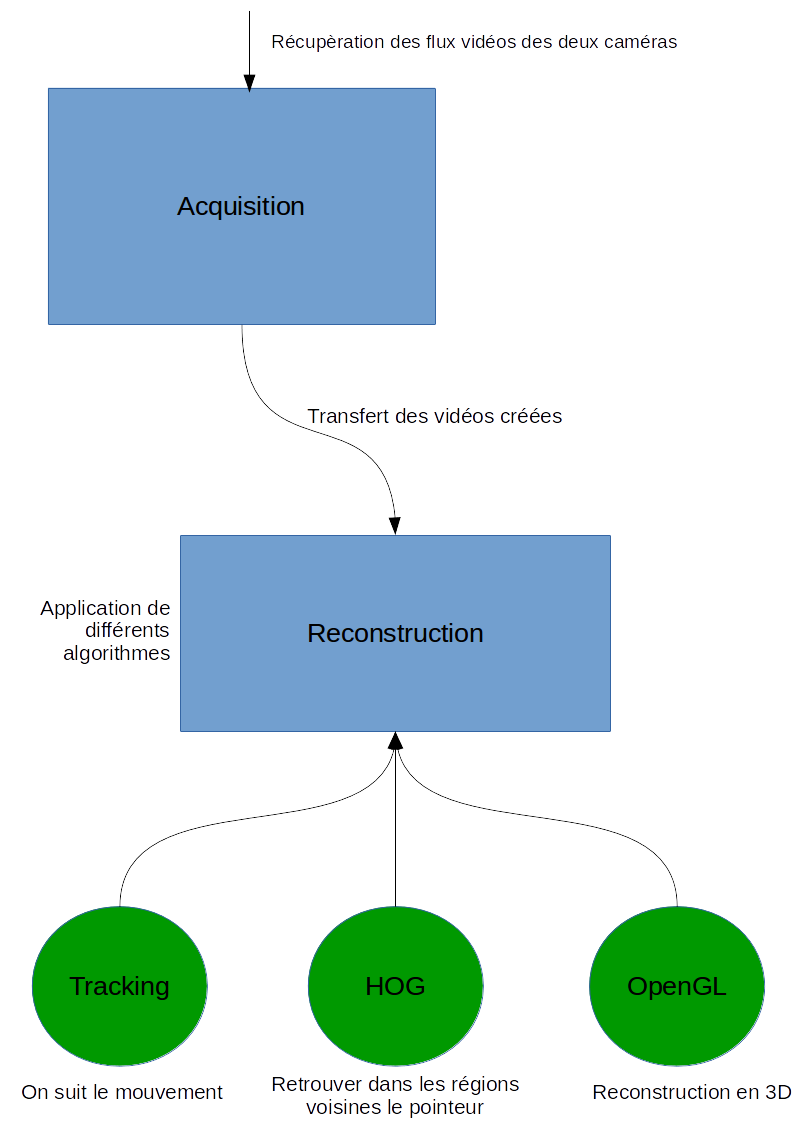
\includegraphics[width=\textwidth]{Modules/Picture/Architecture.png}
\caption{architecture}
\label{architecture}
\end{figure}

\clearpage